\subsection{Conky}
	Conky is going to be configured by a file called conkyrc commonly located in the home directory.
	\subsubsection{Display Configuration}
		\begin{wrapfigure}{l}{0.4\textwidth}
			\begin{center}
				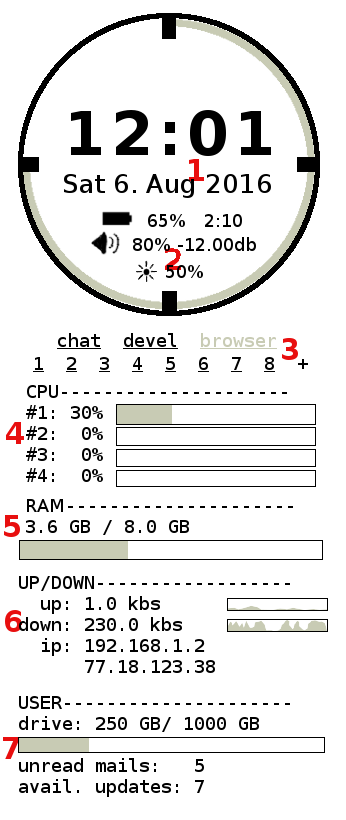
\includegraphics[width=0.40\textwidth]{conky_draft.png}			
			\end{center}
			\caption{conky design draft}
			\label{conky_example}
		\end{wrapfigure}
		
		The conky should look like in the example image \ref{conky_example}. This design covers most requirements.\\
		\\
		Date and time are shown in a circle (nr 1 in image) underneath is the additional battery, volume and brightness information (nr 2). Followed up by the desktop enumeration (nr 3).\\
		CPU and RAM usage are displayed with numbers and bars (nr 4 and 5).\\
		Additionally is the internet speed for up- and download as well as external and internal ip (nr 6) shown. The outdated packages are visible at the end in the user section where also the hard drive capacity is shown (nr 7).\\
		\\
		The text, borders and lines are a light grey (see img \ref{preview}) with the color code of \textbf{7d7d7d}. The filling of graphs, clock and bars is a very light brown with the color code of \textbf{c8cbb4}.
	\subsubsection{Conky Configuration}
		to be able to toggle conky as a HUD with awesome key-bindings the following is required in the conkyrc.
		\begin{lstlisting}
own_window yes
own_window_type desktop
own_window_hints below,skip_taskbar,skip_pager
own_window_colour 000000
own_window_argb_visual yes
own_window_argb_value 110		
		\end{lstlisting}
		
\clearpage
	\subsubsection{Battery, Volume, Brightness}
		The volumen information is easy to access. it will display the percentage and the decibel correction.
		\begin{lstlisting}
${exec amixer -c 0 get Master | grep Mono: | cut -d " " -f6-7}
		\end{lstlisting}
		
		The brightness is read in a similar way. Only the percentage is shown
		\begin{lstlisting}
${exec xbacklight -get | cut -d "." -f1}
		\end{lstlisting}
		
		For the battery is another command required. The remaining battery power in percent and the duration in the format of HH:MM is shown.
		\begin{lstlisting}
${battery_percent} ${battery_time}
		\end{lstlisting}		
		The 3 icons in the table beneath are used.
		\begin{table}[H]
			\begin{tabular}{cl}
				
\includegraphics[width=1cm, height=1cm]{battery.png}
				& Battery icon\tablefootnote{Icon made by \href{http://www.flaticon.com/authors/lucy-g}{Lucy-G} from www.flaticon.com }\\
				
\includegraphics[width=1cm, height=1cm]{speaker.png}			
				& volume icon\tablefootnote{Icon made by \href{http://www.flaticon.com/authors/gregor-cresnar}{Gregor Cresnar} from www.flaticon.com }\\
				
\includegraphics[width=1cm, height=1cm]{sun.png}			
				& brightness icon\tablefootnote{Icon made by \href{http://www.flaticon.com/authors/rami-mcmin}{Rami McMin} from www.flaticon.com }\\
			\end{tabular}
		\end{table}
    
    \subsubsection{Lua clock scripting}
    the round circle with the time and date in it requires a lua script to create the two rings.\\
    \ldots